%% Lee
%% In dissertation, change 
%    section* to chapter 
%    subsection* to section
%    subsubsection* to subsection

% >>>>>>>>>>>>>>>>>>>>>>>>>>>>>>>>>>>>>>>>>>>>>>>>>>>>>>>>>>>>>>>>>>>>>>>>>>>>> DRAM Customizable <<<<<<<<<>>>>>>>>>>>>>>>>>>>>>>>>>>>>>>>>>>>>>>>>>>>>>>>>>><<<<<<<<<<<<<
\chapter{DRAM Customizations}
\label{sec:DRAM Customizations}

There are two types of memory employed in \acp{asic} and \acp{asip}, \acl{sram} or \ac{sram} and \acl{dram}, or \ac{dram}.
Both of these technologies have a similar top level block diagram which contains an array of storage elements, a means to address into a particular row of memory cells and a means to read and write a column of those cells.
A basic block diagram is shown in figure \ref{fig:MemoryBlockDiagram}.
\begin{figure}[!t]
% the [] contains position info e.g. [!t] means here
\centering
\captionsetup{justification=centering}
\centerline{
\mbox{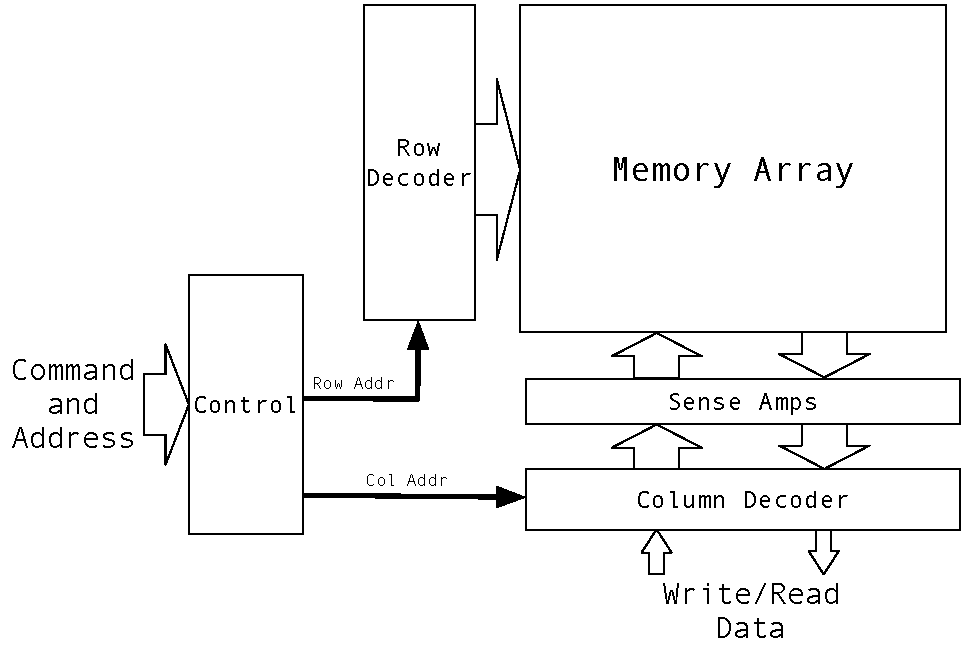
\includegraphics[width=.8\linewidth]{BasicMemoryBlockDiagram}}
}
\caption{Typical Memory Block Diagram \cite{Jacob:2007:MSC:1543376}}
\label{fig:MemoryBlockDiagram}
\end{figure}


\begin{figure}
\centering
\begin{subfigure}{.45\textwidth}
  \centering
  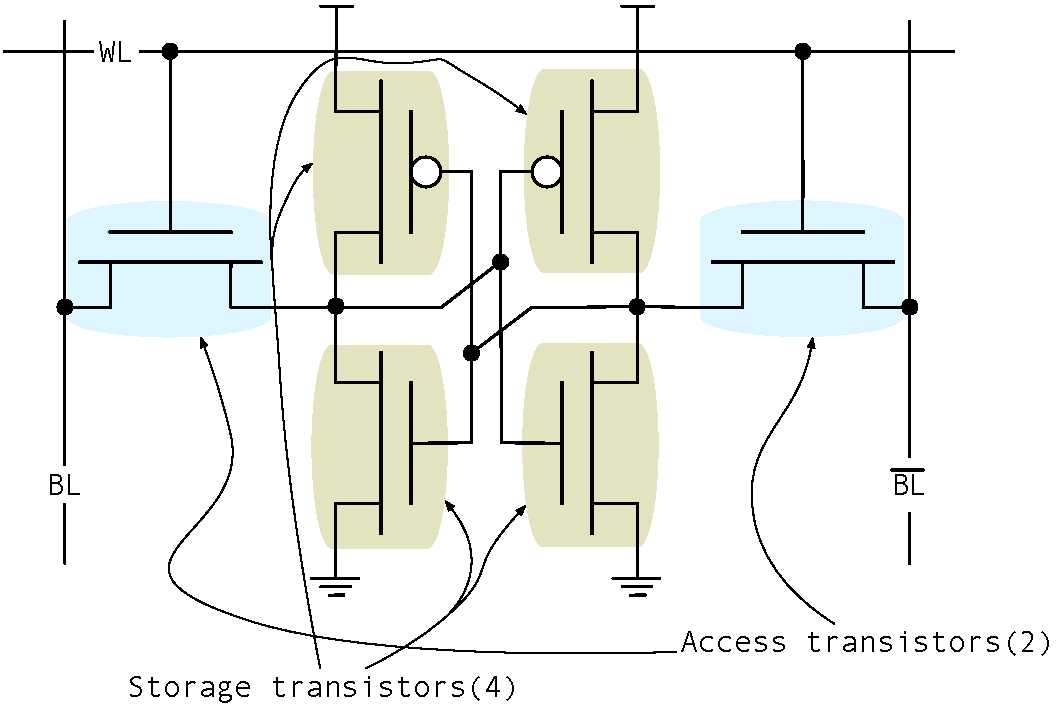
\includegraphics[scale=0.4]{SRAM_Cell}
  \captionsetup{justification=centering, skip=5pt}
  \vspace{-6pt}
  \caption{SRAM Storage Cell \cite{Jacob:2007:MSC:1543376}}
  \label{fig:SRAM Cell}
\end{subfigure}%
\begin{subfigure}{.45\textwidth}
  \centering
  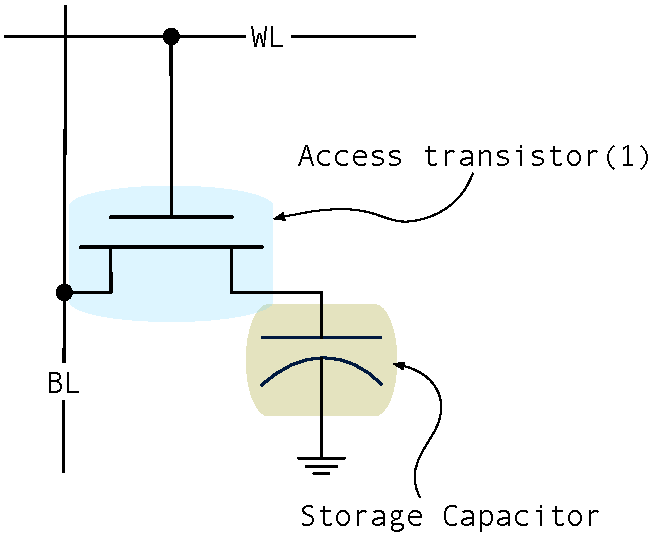
\includegraphics[scale=0.4]{DRAM_Cell}
  \captionsetup{justification=centering, skip=5pt}
  %\vspace{36pt}
  \vspace{20pt}
  \caption{DRAM Storage Cell \cite{Jacob:2007:MSC:1543376}}
  \label{fig:DRAM Cell}
\end{subfigure}
\captionsetup{justification=centering, skip=12pt}
\caption{RAM Storage Cell Types}
\label{fig:Memory Storage Cells}
\end{figure}


Accessing a typical \ac{sram} involves providing an address and either reading or writing the contents of that location. 
The read or write often completes in one or two clock cycles depending on whether the \ac{sram} employs internal registers which are used run the \ac{sram} with a faster clock.

The storage cell inside the \ac{sram} is formed from cross-coupled transisters (see figure \ref{fig:SRAM Cell}) which latch the contents and hold the contents indefnitely or until power is removed from the device.
The storage structure employs six transistors and allows the access logic to be relatively simple and fast but has a relatively low XXXXXXXXXXXX capacity.

Accessing a "typical" DRAM is much more involved, it involves opening a page in a bank, reading or writing a portion of the contents of the page then closing the page. 

The reasons behind this added complexity is the memory cell inside the \ac{dram} which is formed from a capacitor (see figure \ref{fig:DRAM Cell}) which holds a charge reflecting a logic zero or one. 
The major difference between the \ac{sram} cell is the number of elements it takes to implement. The size of the \ac{dram} cell means \ac{dram} arrays provide five to six times more storage when compared to a similar sized \ac{sram} array.
The major disadvantage is the capacitor cannot hold a indefnitely because the leakage currents in \acp{ic} cause the charge to leak away. If kept unchecked, the stored value will dissipate and it is this behavior that makes accessing a \ac{dram} array more complicated than a similar \ac{sram} array.

When an \ac{sram} cell is read, the cross-coupled transistors retain the stored value. The issue with \acp{dram} is when a storage cell is read, the capacitor is discharged. In addition, sensing this discharging capacitor takes long time to sense when compared to the \ac{sram} cell.
To alleviate this problem, \ac{dram} arrays are formed from a column of storage elements known as a page. When the read occurs, the entire contents of the page are transferred to registers. Once this transfer is complete, portions of the page can be read similar to reading an \ac{sram}. 
The problem is that if another read wants to access data that is not in the page, the page has to be closed and another page opened. This involves transferring the previously registered page back to the array to recharge the capacitors in the pages storage elements. The next page can then be read and transferred to the page registers.
The process of opening and closing pages is a relatively long time, typically 10-20\SI[per-mode=symbol]{}{\nano\second}. So if the accesses are somewhat random, accesses are very slow when compared to \ac{sram}.
To get around this issue, the \ac{dram} is formed from more than one array of storage elements, between 8 and 32, know as banks. The idea is that while a page from one bank is being accessed, another bank can be opened in preparation for a future read (or write).
This access protocol is rather complicated and if consequtive accesses are not sequenced carefully, the performance of \ac{dram} can be poor.

The sequence of accesses cannot always be controlled, especially in general purpose computers, so \ac{sram} is typically used as the first level of memory with \ac{dram} used as the primary storage. 
using \ac{sram} as this first level memory is called a cache and these have been used for decades to isolate the computing system from unpredictable access behavior of the \ac{dram}.

As mentioned in section \ref{sec:overview} much of the \ac{asic} and \ac{asip} \ac{ann} research has focused on taking advantage of the performance and ease of use of \ac{sram}, but with this works target application an \ac{asic} or \ac{asip} employing \ac{sram} as its primary memory cannot be implemented with adequate storage capacity.
Under these circustances, \ac{dram} bandwidth will be the bottleneck.

This work focuses on using \ac{dram} as the primary storage and managing the accesses to ensure the \ac{dram} is used effectively. 
With the additional \ac{dram} customizations discussed in section \ref{sec:Very-Wide Bus} and \ref{sec:Write Mask}, this work demonstrates \ac{dram} bandwidths 10X faster than what is available with 2 or 2.5D solutions.
This high level of \ac{dram} bandwidth provides this work the ability to process multiple disparate \acp{ann} at or near real-time whilst being \textbf{\textcolor{black}{10-100X faster than state-of-the-art solutions}}.


\section{Customization One: Very-Wide Bus}
\label{sec:Very-Wide Bus}

Typically a bank may contain of the order of a few thousand pages and a page may contain of the order of a few thousand bits.

Once the page is open, the user accesses a portion of the requested page over a bus. With PCB based DRAMs the bus might vary from four to 16 bits wide, but with 3D DRAMs, such as HBM the bus might be up to 128 bits wide.

Figure \ref{fig:dramBlockDiagram} shows a block diagram of a typical DRAM.

\begin{figure}[!t]
% the [] contains position info e.g. [!t] means here
\centering
\captionsetup{justification=centering}
\centerline{
\mbox{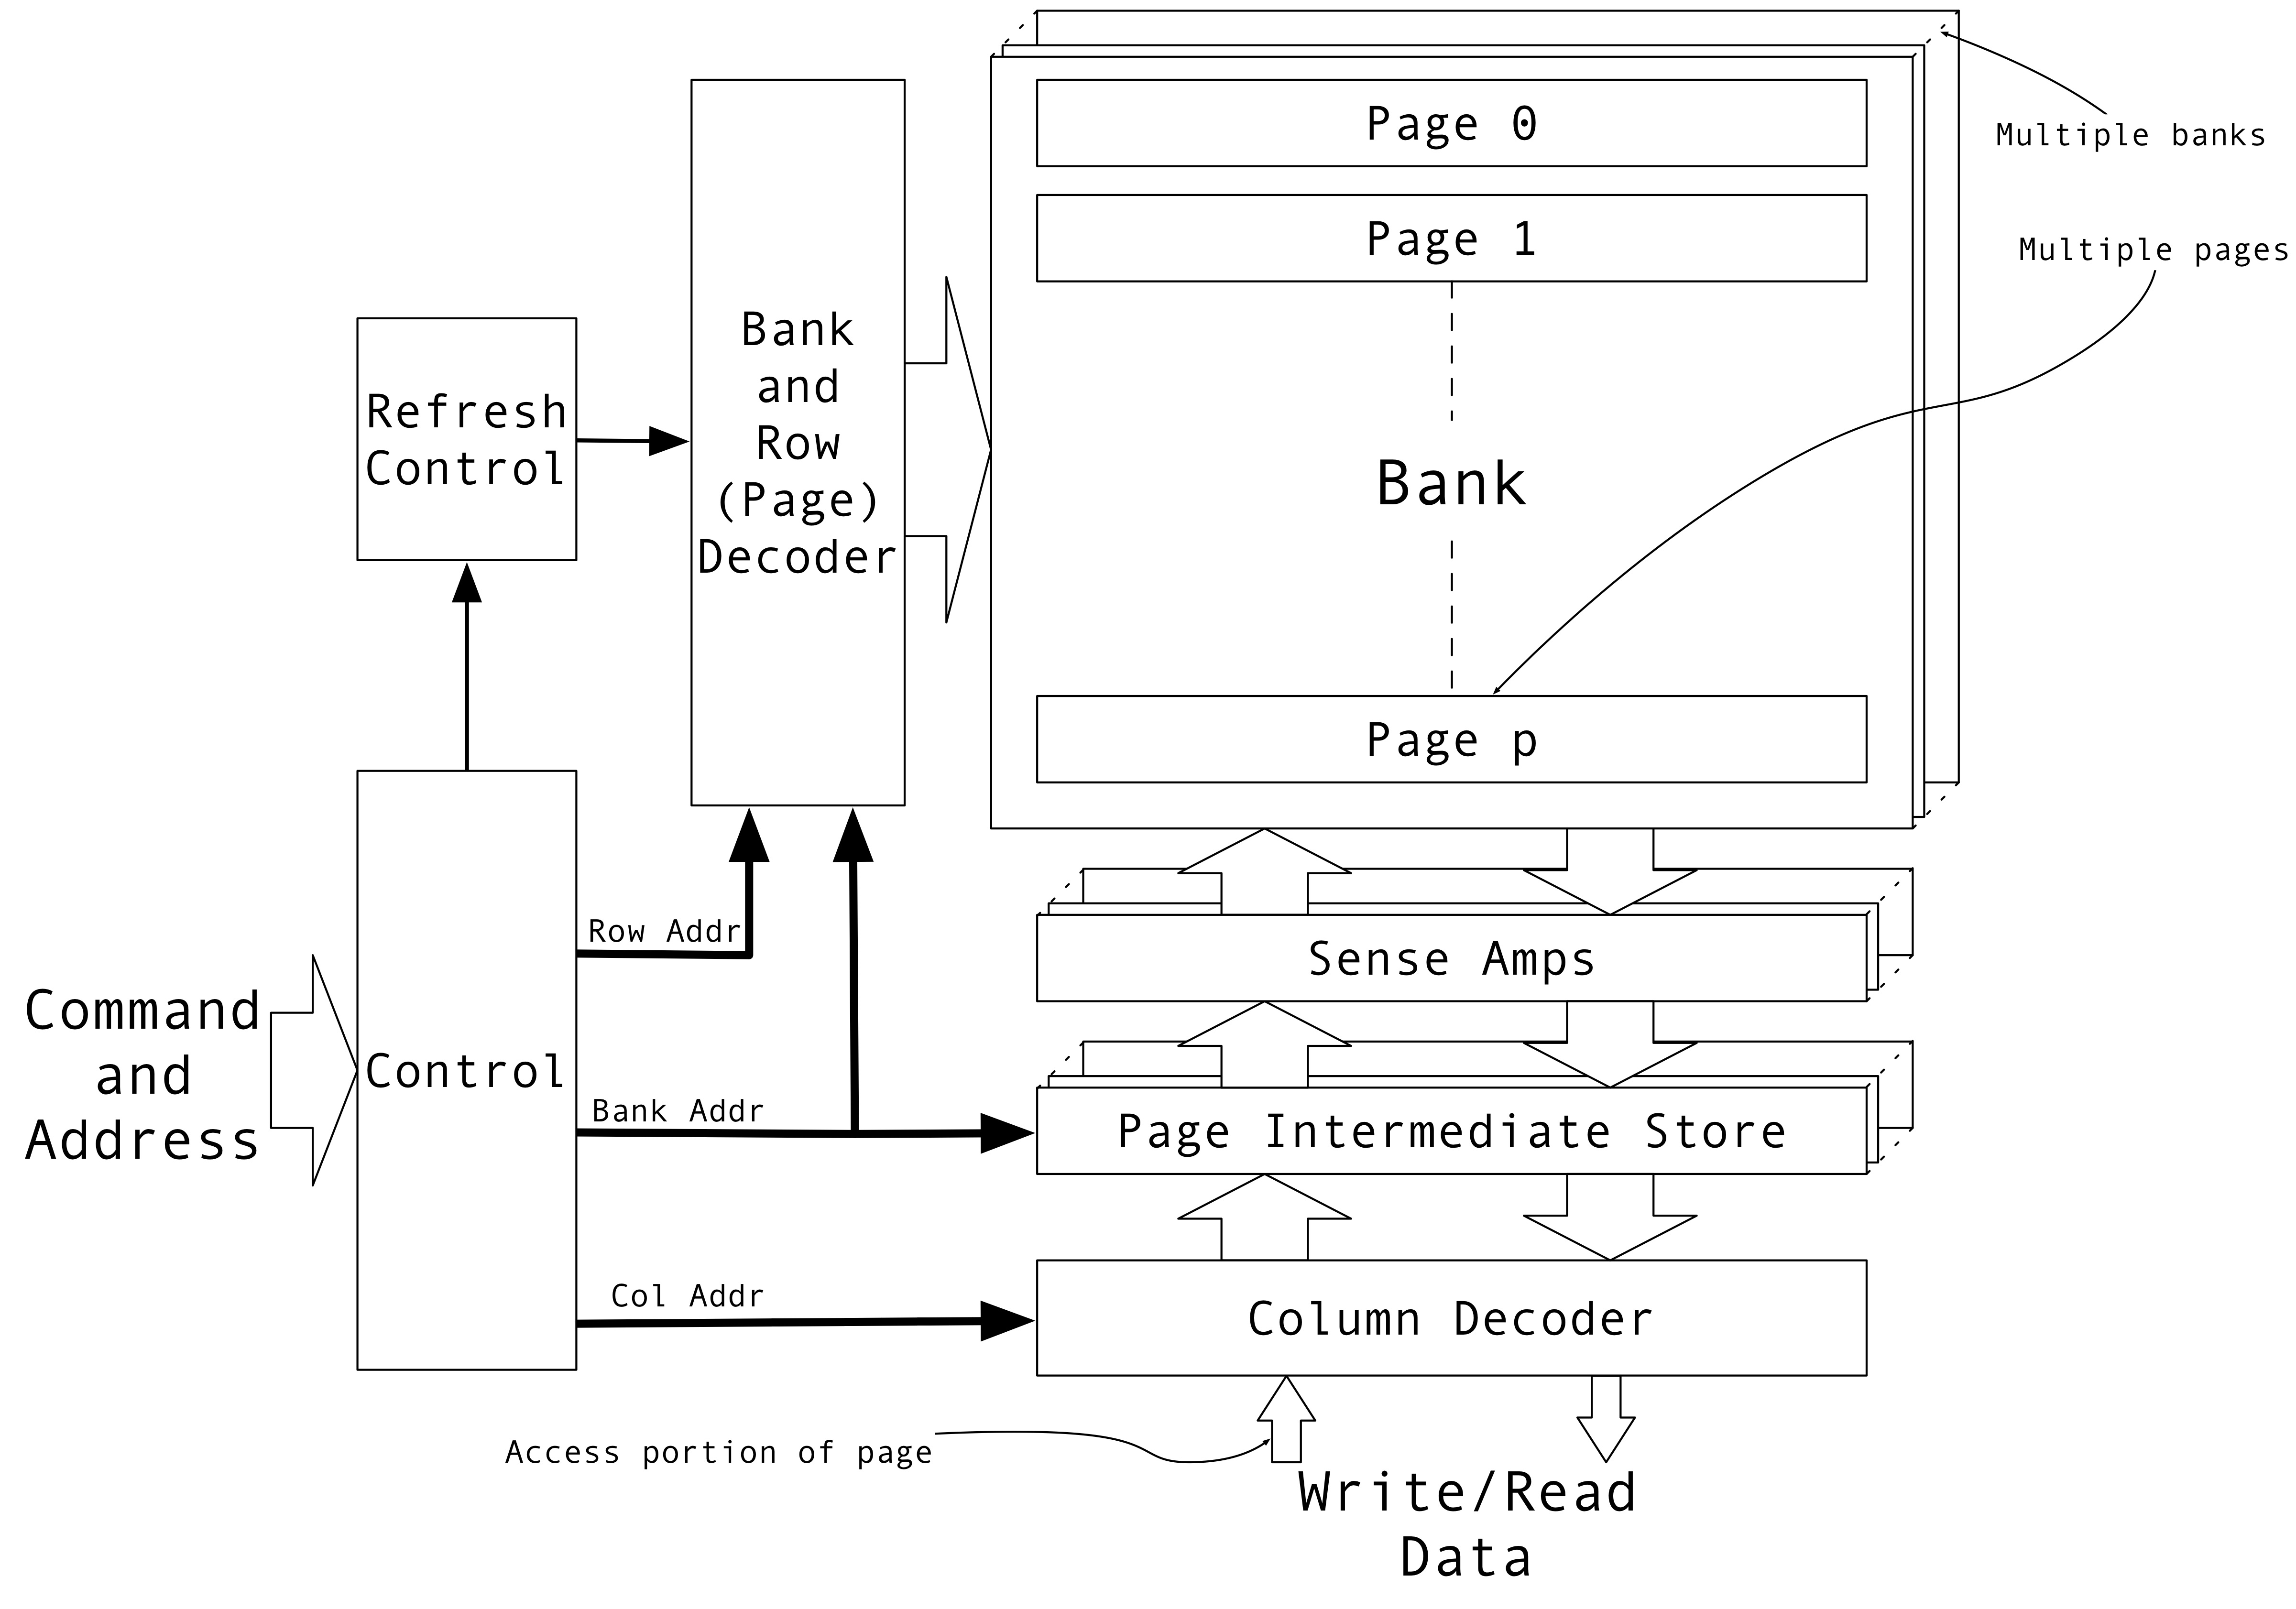
\includegraphics[width=.75\linewidth]{DRAMBlockDiagram.jpg}}
}
\caption{Typical DRAM Block Diagram}
\label{fig:dramBlockDiagram}
\end{figure}

This work achieves the increase in bandwidth by proposing that the DRAM expose more of its currently open page.

Without the limitations of having to transfer data beyond the chip stack, this work suggests exposing a larger portion of the page over a very wide bus. By staying within the 3D footprint, this bus can be implemented using fine pitch through-silicon-vias.
(see figure \ref{fig:dramBusChange}).

\begin{figure}[!t]
% the [] contains position info e.g. [!t] means here
\centering
\captionsetup{justification=centering}
\captionsetup{width=.75\linewidth}
\centerline{
\mbox{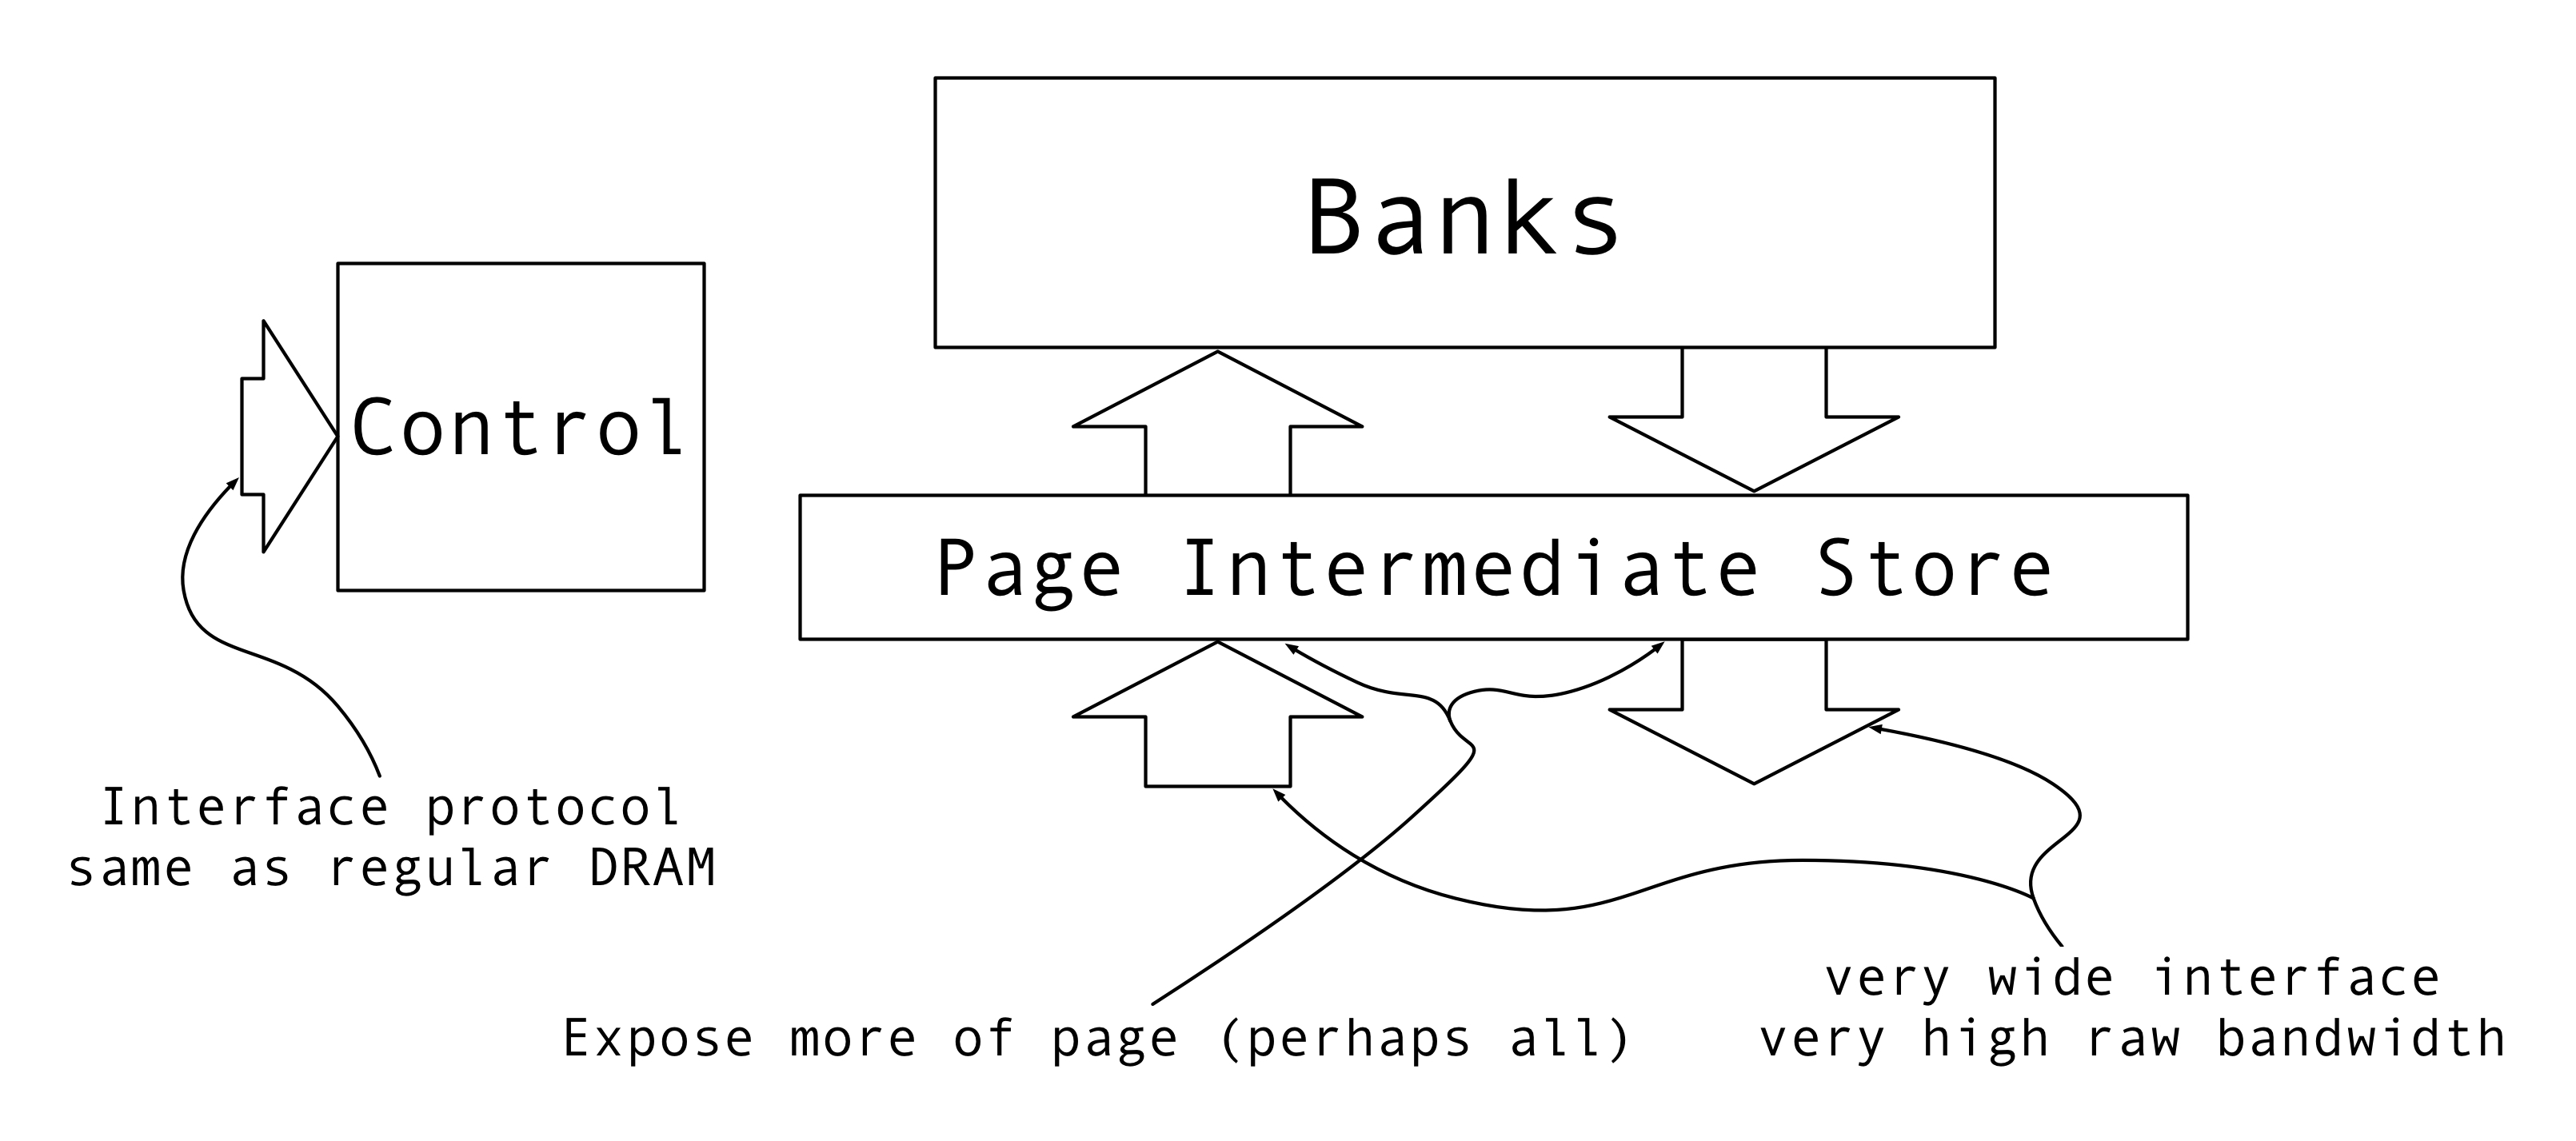
\includegraphics[width=.65\linewidth]{DRAMBusChange.jpg}}
}
\caption{Exposing more of the DRAM page}
\label{fig:dramBusChange}
\end{figure}

This work assumes the \ac{dram} interface protocol uses \ac{ddr} with a bus width of 2048. Given the \ac{diram4} employs a burst of two for read and write cycles, an entire \ac{diram4} page of 4096-bits is accessed during each read or write. 

\section{Customization Two: Write Mask}
\label{sec:Write Mask}
When processing an ANN, to compute the activation of an individual AN involves reading the pre-synaptic AN activations and the weights of the connections between the pre-synaptic ANs and the AN being processed. The activation of the processed AN is written back to memory. The ratio of reads to writes is high, 100s or 1000s to one. Therefore, the system often needs to write a portion of the page back to memory. To avoid a read/modify/write, a customization to the DRAM is the addition of a write data mask to the DRAM write path.

This work assumes single precision floating point for \ac{ann} weights and activation, so a mask bit will be provided on a word basis or every 32-bits.

